
\section{MSC}
\label{sc:MSC}
MSC ist von der International Telecommunication Union (ITU) normierte Sprache.  Sie hat eine graphiseche Notation, um den Benutzer zu darstellen, und eine textuelle Notation für die Bearbeitung durch Software-Werkzeuge, genauso wie bei SDL.
MSC bietet die Möglichkeit, das Kommunikationsverhalten zwischen Systemkomponenten und deren Umgebung zu beschreiben. Diese Kommunikations ist auf den Austaush von Nachrichten basiert.
Mit Msc-Specifikationen können unterschiedliche Sichten auf das Systemverhalten erzeugt werden. 
Dazu gibt MSC einen globalen Einblick auf das System aus, wie zum Beispiel die Interaktionen von alle Instanzen.\\
MSC und UML haben fast das gleiche Prinzip und man kann sogar als Variante von MSC den Sequence Diagrams in UML integrieren.
Trotz der vielen Gemeinsamkeiten von dieser drei Modellierungssprachen (UML, SDL und MSC), haben sie viele große Unterschied in dem tatsächlichen Entwurf. Beispielsweise kann man mit MSC nur Beispielabläufe und kein vollständig System beschreiben.\\
Die MSC-Diagramme sind in den frühen Phasen hilfreich, wobei können sie erste Ideen und Einblick zum System anzeigen.
Damit kann man einfach in der Entwurfsphase wichtige erwünschte oder unerwünschte Beispielabläufe bemerken oder in späteren Phasen den Testzweck schauen, der von die MSC-Diagramme genau definiert wurde.\\

Die wichtigsten Konstrukte und Elemente der MSC werden in diesem Abschnitt anhand ein Beispiel dargestellt. Wir glauben, dass ein Beispiel das beste Weise ist, um Das MSC Konzept zu erklären und zu definieren. 
Das folgende Beispiel beschreibt einen Prozess, der aus vier verschiedenen Einzelteilen (A, B, C und D) zwei Produkte von Typ AC oder BDC produziert. 


\subsection{Basic-MSC}
Das erste wichtige Teil von MSC ist ein Basic-MSC. Ein Basic-MSC umfasst alle notwendige Srachkonstrukte zur Spezifizierung des Nachrichtenfluss.
Die Sprachkonstrukte von einem einfachen MSC (Basic MSC9 sind: Instanz, Message, Environment, Action, Timer-Start, Timeout, Timer-Stop, Create, Stop und Condition. \\
Das wichtigste Teil vom Basic-MSC sind den Nachrichtenaustausch. Diese Nachrichten können verschiedene Parameter tragen, die den Typ einer Nachricht unterscheiden. Auf dieser Weise sind zwei Nachrichten gleich, wenn sie den gleichen Inhalt besitzen.
Ein Basic-MSC definiert eine partielle Ordnung auf Ereignissen, die an einem Ort (heißt Instanz) stattfinden.
Diese Ereignissen können in verschiedenen Fromen erscheint werden, zum Beispiel: Kommunikationsereignisse ( wie das Senden und Empfangen einer Nachricht), Timer-Ereignisse, lokale Aktionen oder das Erzeugen einer Instanz.\\
Um ein Basic-MSC besser zu erklären, ist ein Beispiel davon in der nächsten Abbildung gezeigt.
Ein Basic-MSC mit dem Namen ProduktionAC ist in
Abbildung 1.6 gezeigt.
\begin{center}
\begin{figure}[h]
   

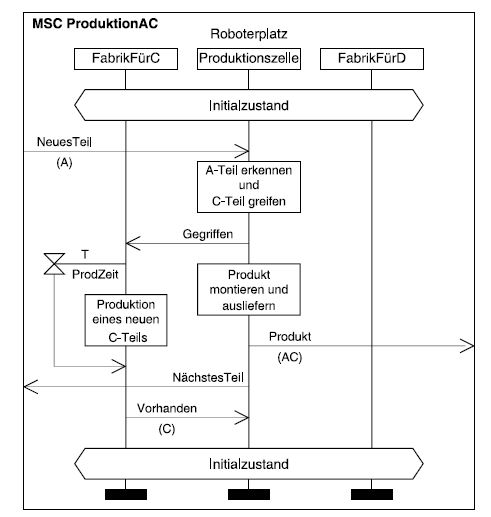
\includegraphics[scale=1]{Graphics/MSC1.jpg}

\captionof{figure}{Ein Basic-MSC}


Quelle : \cite{MT009}
Part 1: Message Sequence Chart (MSC) 

 
\label{fig7}


\end{figure}

\end{center}
\newpage
Der Name von diesem Basic-MSC ist ProduktionAC und er muss oben in der Ecke geschrieben werden. Das Basic-MSC in diesem Beispiel beschreibt die Produktion eines Produkts, das aus einem A-Teil und einem C-Teil zusammengesetzt ist.
Die wichtige Elemente in dieser Abbildung sind: Der Produktionszelle, FabrikfürC und Fabrik von D. Das MSC beschreibt ein detaillierte Szenario vom Informationsaustausch zwischen diese drei Element. 

\\
Am Anfang ist der Produktionsprozess in seinem Initialzustand, Der ein benötige Bedingung für die nächste Aktionen ist. 
 Das System ist initialisiert und Teile
der Typen C und D sind gefertigt, eingelagert und der
Produktionszelle zur Verfügung gestellt worden.
 Die Systemumgebung schickt das A-Teil an die Produktionszelle.
 Danach erkennt die Produktionszelle das empfangende Teil, greift das für die Produktion notwendige C-Teil und meldet das Entfernen des
 C-Teils vom Greifplatz an die FabrikfürC, die für das C-Teile zuständig ist. 
 Beim letzten Schritt wird ein Produkt von Typ AC produziert, ausgegeben und zu die Systemumgebung geschickt.
Danach meldet die Produktionszelle die Bereitschaft
für die Bearbeitung des nächsten A- oder B-Teils
an die Systemumgebung.
In der Gleichzeitig wird ein neues C-Teil wieder produziert und es ist jetzt verfügbar für die nächste Produktion.

\subsubsection{Instanz und Message}
Instanzen und Nachrichten (Message) sind die wichtigste Sprachkunstrukte von Basic-MSC.

Instanzen sind Komponenten, die mit der Systemumgebung oder untereinander
asynchron Nachrichten austauschen können.\\
Die Instanzen sind als vertikale Linien dargestell. Am Enfang dieser Linier findet man der Instanzkopf, wo der Instanzname spezifiziert wird. Zusätzlich kann man noch direkt über den Instanzkopf ein Typ zu dieser Instanz angeben (z.B. Instanz Produktionszelle vom Typ Roboterplatz in Abbildung).
Die Linie der Instanzen endet sich mit einem Instanz-Ende-Symbol. Ein Instanz-End bedeutet, dass es in dem MSC keine weiteren Ereignisse für diese Instanz gibt, aber das bedeutet nicht unbedingt, dass die Instanz gestoppt ist.\\


Die Nachrichten werden durch Pfeile dargestellt. Die Pfeile
können horizontal oder geneigt sein, um den Zeitverlauf
anzuzeigen. 
Jede Nachricht definiert definiert genau zwei Eereignisse: Das Senden der Nachricht ist durch den Pfeileanfang beschrieben und die Pfeilspitze bezeichnet
die Verarbeitung einer Nachricht.
Jede Nachricht hat einen Name und optionale Nachricht-Parametern, die in Klammern angegeben werden müssen (Zum Beispiel in Abbildung hat die erste Nachricht den Name NeuesTeil mit dem Parameter A).
 Bei Jeder Instanzlinie gibt es eine Totalordnung der der spezifizierten
 Message-Sende- und Message-Verarbeitungsereignisse. Dazu gibt es zwischen die verschieden Instanzachse partiell Ordnung, wobei sollte eine Nachricht zuerst gesendet werden, bevor sie empfängt wird. 

\subsubsection{Environment}
Die Systemumgebung ist durch die Diagrammfläsche eines MSC definiert. Diese Diagrammfläsche wird durch einen rechteckigen Rahmen begrenzt.
die Systemumgebung und heißt Environment. Nachrichten,
die aus der Systemumgebung kommen oder an die Systemumgebung
gesendet werden, beginnen und enden auf
dem Environment (z.B. die Messages NeuesTeil und
Produkt in Abbildung). Die Sende- und Verarbeitungsereignisse aus und an die Systemumgebung definieren in der Regel keine Ordnung.

\subsubsection{Action}

Aktionen von Instanzen können ind Form von Actions spezifiziert werden.
Eine Action wird durch ein Rechtecksymbol dargestellt, der Name der Aktion enthalten kann (z.B. Action ,Produkt
montieren und ausliefern‘ in Abbildung).
\\
\subsubsection{Timer}
Die Sprachkonstrukte Timer-Start, Timeout und Timer-Stop können zusätzlich die Timern beschreiben, damit wird es deutlicher den Anfang und das Ende der Aktionen definiert.
Der Anfang der Pfeile(mit Sanduhr-Symbol) definiert das Time-Start und das Ende der Pfeile definiert das Timeout. Zusätzlich muss man den Name von Timer und optional die Timer-Parametern definieren.

Ein Timer-Start und seine Timeout werden
in Bild Abbildung verwendet, um die Produktionszeit für ein Teil des
Typs C zu modellieren.In diesem Fall hat der Timer hat den Namen T und
den Parameter Prodzeit.\\
\subsubsection{Condition}
Die Beschreibung vom Zustand definiert durch Condition ( Bedingung)
Graphisch werden Conditions durch Sechsecke dargestellt,
die die Instanzen, auf die sich die Condition bezieht,
überdecken. Conditions werden zur Beschreibung von
wichtigen Systemzuständen benutzt. In Abbildung befinden sich
zwei Conditions, die Initialzustand heißt und den globalen Systemzustand beschreiben.\\


\subsection{Strukturelle Sprachkonstrukte}
Strukturelle MSC-Sprachkonstrukte bezeichnen Sprachelemente,
die über die Beschreibung des reinen Messageflusses
hinausgehen. Mit ihnen lassen sich MSCs und
MSC-Teile zu komplexeren Abläufen kombinieren (Inline-
Expressions und High-Level-MSC), MSC-Diagramme in
anderen MSC-Diagrammen wiederverwenden (References),
MSC-Instanzen verfeinern (Decomposition) und allgemeine
Ereignisstrukturen für Instanzen definieren (Coregion und
General Ordering).\cite{MT009}\\

\begin{center}
\begin{figure}[h]
   

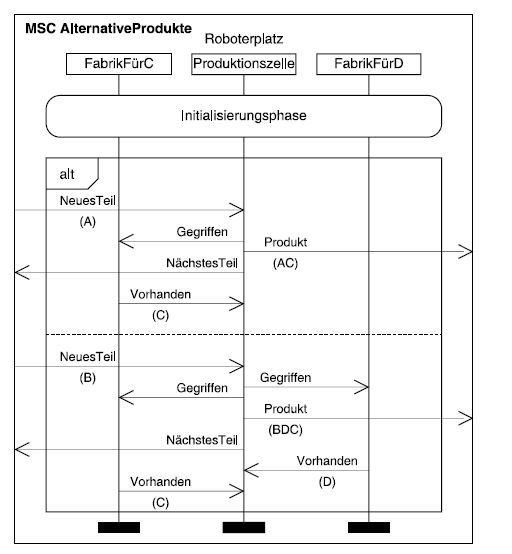
\includegraphics[scale=1]{Graphics/MSCmit.jpg}

\captionof{figure}{MSC mit strukturellen Sprachkonstrukten }


Quelle : \cite{MT009}
Part 1: Message Sequence Chart (MSC) 

 
\label{fig8}


\end{figure}

\end{center}
\newpage
\subsubsection{Inline-Expressions}
Inline-Expression werden als Operatoren in MSCs definiert. Damit können Teilabläufe,
die innerhalb eines MSC-Diagramms spezifiziert worden sind, zu komplexeren Abläufen kombiniert werden. Sie erlauben es, die Wiederholung von Teilabläufen (loop-Operator),
alternative Teilabläufe (alt-Operator), die parallele Komposition von Teilabläufen (parOperator), optionale Teilabläufe (opt-Operator) und Ausnahmen in Form von Teilabläufen (exc-Operator) zu spezifizieren. Graphisch werden Inline-Expressions als Rechtecke mit in der linken oberen Ecke spezifizierten Namen dargestellt. Teilabläufe werden durch gestrichelten Linien in Sections separiert.
\subsubsection{References}
References ermöglichen es, MSCs in anderen MSCs wieder
zu verwenden. 
Ein Reference unterscheidet und referenziert die andere MSC mit dessen Namen. 
Die References sind mit abgerundeten Rechteck dargestellt (z.b Ein Reference ist mit dem Name Initialisierungsphase in Abbildung dargestellt).\\


\subsection{High-Level-MSC}
High-Level-MSC ist auch als (HMSC) bekannt. Es ermöglicht eine kombinierte Darstellung von mehren MSCs auf abstrakter Ebene. Diese Kombination ist durch gerichteten Graphen beschriebt. Die Knoten eines HMSC-Diagramms sind ein Anfangsknoten, Endknoten, Konnektoren, References und Conditions.
\\ HMSC gibt ein globale Einblick von der gesamten Kombination von MSC-Diagrammen, damit kann man parallele, sequentielle alternative
Kombination von MSCs in einer Einzige Abbildung und in einer sehr intuitiven Form beschreiben.\\•



\begin{center}
\begin{figure}[h]
   

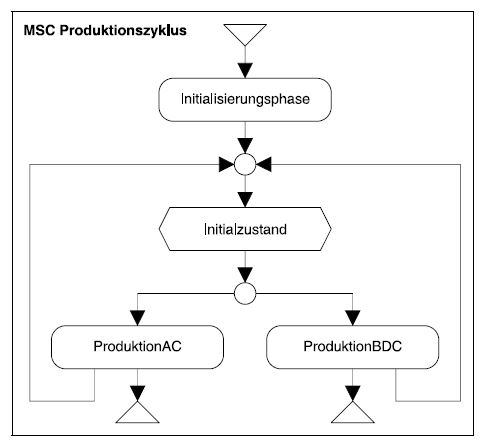
\includegraphics[scale=1]{Graphics/HMSC.jpg}

\captionof{figure}{Ein High-Level-MSC }


Quelle : \cite{MT009}
Part 1: Message Sequence Chart (MSC) 

 
\label{fig9}


\end{figure}

\end{center}
\newpage
In der Abbildung beschreibt das HMSC-Beispiel, die verschiedene Szenarien, die im Produktionsprozess-Beispiel passieren können. 
Die verschieden Szenarien in dieser Abbildung sind:Am Anfang gibt es direkt die Initialisierungsphase,danach
befindet sich der Produktionsprozess in seinem
Initialzustand. Im Initialzustand können entweder Produkte
vom Typ AC oder vom Typ BCD hergestellt werden. Nach
der Herstellung eines Produkts befindet sich der Produktionsprozess
wieder im Initialzustand und ein neues Produkt
kann entweder gefertigt werden oder der Produktionsprozess endet.

\subsection{Weitere Sprachkonstrukte}
Wir haben in diesem Abschnitt dieses Kapitel nur an die sichtigsten Elemente der MSC-Sprache konzentriert. Damit haben wir ein globale aus ausreichende Einblick, um diese Modellierungssprache zu bewerten. Aber dazu gibt es noch weitergehende Konzepte, die MSC zu einer vollständigen Spezifikationssprache machen






